\examxtitle{浙江省金华十校2025-2026学年高三上学期一模}

\section{单选题}

\begin{question}
已知集合 \(U=\{1,2,3,4,5,6,7,8\}\) , \(A=\{2,3,4\}\) ,则集合 \(\complement_{U}A=\)()
\begin{choices}
  \item \(\{1\}\)
  \item \(\{2,3,4\}\)
  \item \(\{5,6,7,8\}\)
  \item \(\{1,5,6,7,8\}\)
\end{choices}
\topics{补集的概念及运算}
\difficulty{0.94}
\answer{D}
\explain{由\(U=\{1,2,3,4,5,6,7,8\}\),\(A=\{2,3,4\}\),则\(\complement_{U}A=\{1,5,6,7,8\}\)}
\end{question}

\begin{question}
已知等差数列\(\{a_{n}\}\)满足\(a_{1}=2\),\(a_{4}+a_{6}=20\),则\(a_{3}=\)()
\begin{choices}
  \item 4 
  \item 6 
  \item 8 
  \item 10
\end{choices}
\topics{等差中项的应用}
\difficulty{0.85}
\answer{B}
\explain{由题设\(a_{4}+a_{6}=2a_{5}=20\Rightarrow a_{5}=10\),而\(a_{1}=2\), 所以\(a_{1}+a_{5}=2a_{3}=12\Rightarrow a_{3}=6\)}
\end{question}

\begin{question}
\(\frac{5}{2+i}=\) ( )
\begin{choices}
  \item \(2+i\)
  \item \(2-i\)
  \item \(-2+i\)
  \item \(-2-i\)
\end{choices}
\topics{复数代数形式的乘法运算;复数的除法运算}
\difficulty{0.85}
\answer{B}
\explain{\(\frac{5}{2+i}=\frac{(2+i)(2-i)}{2+i}=2-i\)}
\end{question}

\begin{question}
已知\(\frac{1}{\log_{9}a}+\frac{1}{\log_{27}a}=\frac{5}{3}\),则\(a=\)()
\begin{choices}
  \item 3 
  \item 9 
  \item 27 
  \item 81      
\end{choices}
\topics{指数幂的运算;指数式与对数式的互化;对数的运算;运用换底公式化简计算}
\difficulty{0.65}
\answer{C}
\explain{\(\frac{1}{\log_{9}a}+\frac{1}{\log_{27}a}=\log_{a}9+\log_{a}27=\log_{a}3^{5}=\frac{5}{3}\),所以\(a^{5}_{3}=3^{5}\),则\(a^{5}=(3^{5})^{3}=27^{5}\),解得\(a=27\)}
\end{question}

\begin{question}
已知随机变量 \(X\sim N\left(2, \sigma^{2}\right)\) ,且 \(P\left(X<0\right)=0.3\) ,则 \(P\left(0<X<4\right)\) 的值为( )
\begin{choices}
  \item 0.2
  \item 0.4
  \item 0.7
  \item 0.35
\end{choices}
\topics{指定区间的概率}
\difficulty{0.65}
\answer{B}
\explain{由题设\(P(X<2)=0.5\),且\(P(X<0)=0.3\),则\(P(0<X<2)=0.2\),由正态分布曲线关于\(X=2\)对称,则\(P\big(0<X<4\big)=0.4\)}
\end{question}

\begin{question}
若圆C:\((x-1)^{2}+(y+3)^{2}=1\)上存在两点A,B,直线l:\(3x-4y+m=0\)上存在点P,使得 \(\angle APB=60^{\circ}\) ,则实数m的取值范围为( )
\begin{choices}
  \item \([-25,-5]\)
  \item \((-\infty,-25)\cup[-5,+\infty)\)
  \item \([-35,5]\)
  \item \((-\infty,-35)\cup[5,+\infty)\)
\end{choices}
\topics{求点到直线的距离;由直线与圆的位置关系求参数}
\difficulty{0.15}
\answer{A}
\explain{当直线与圆相交时,如图所示,若 \(A\)、\(B\) 离直线越近时,直至与直线和圆 \(C\) 的两交点重合,此时 \(\angle APB=\pi\), 若 \(A\)、\(B\) 相距越来越近时,直至 \(A\)、\(B\) 两点重合,此时 \(\angle APB=0^{\circ}\), 所以一定存在 \(A\)、\(B\) 及 \(P\),使得 \(\angle APB=60^{\circ}\);
\begin{center}
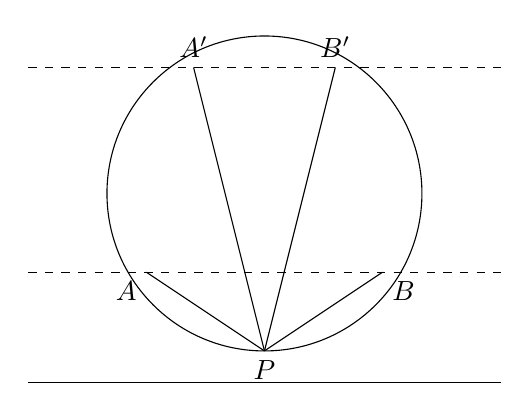
\begin{tikzpicture}[>=stealth,scale=1]
  % circle
  \coordinate (P) at (0,-2);
  \coordinate (O) at (0,0);
  \draw (O) circle (2);
  % horizontal lines
  \draw (-3,-2.4)--(3,-2.4);            % bottom solid
  \draw[dashed] (-3,-1)--(3,-1);        % lower dashed inside
  \draw[dashed] (-3,1.6)--(3,1.6);      % upper dashed
  % points on circle
  \coordinate (A)  at (-1.5,-1);
  \coordinate (B)  at ( 1.5,-1);
  \coordinate (Ap) at (-0.9, 1.6);
  \coordinate (Bp) at ( 0.9, 1.6);
  % radii from P
  \draw (P)--(A);
  \draw (P)--(B);
  \draw (P)--(Ap);
  \draw (P)--(Bp);
  % labels
  \node[below] at (P) {$P$};
  \node[below left]  at (A)  {$A$};
  \node[below right] at (B)  {$B$};
  \node[above] at (Ap) {$A'$};
  \node[above] at (Bp) {$B'$};
\end{tikzpicture}
\end{center}
当直线与圆相切时,同直线与圆相交分析可知,一定存在 \(A\)、\(B\) 及 \(P\),使得 \(\angle APB=60^{\circ}\);当直线与圆没有公共点时,对直线上的任一点 \(P\),若 \(A\)、\(B\) 相距越来越近时,直至 \(A\)、\(B\) 两点重合时,仍有 \(\angle APB=0^{\circ}\),另一方面,若 \(PB\) 与圆 \(C\) 相切于 \(B\),\(PA\) 与圆 \(C\) 相切于 \(A\),此时 \(\angle APB\) 必为该 \(P\) 点所能达到的最大情况,如图所示,
\begin{center}
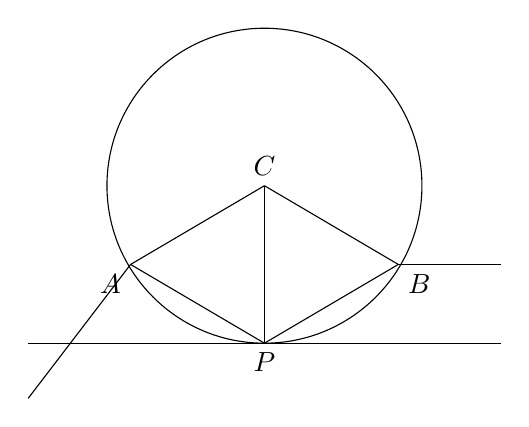
\begin{tikzpicture}[>=stealth,scale=1]
  % horizontal tangent line
  \draw (-3,-2)--(3,-2);
  % circle
  \coordinate (C) at (0,0);
  \draw (C) circle (2);
  % point P on line and circle
  \coordinate (P) at (0,-2);
  % tangent lines from P
  \coordinate (A) at (-1.7,-1);
  \coordinate (B) at ( 1.7,-1);
  \draw (-3,-2.7)--(A);   % left tangent extension
  \draw (3,-1.0)--(B);    % right tangent extension
  % radii and chords
  \draw (C)--(P);
  \draw (C)--(A);
  \draw (C)--(B);
  \draw (P)--(A);
  \draw (P)--(B);
  % labels
  \node[below] at (P) {$P$};
  \node[below left]  at (A) {$A$};
  \node[below right] at (B) {$B$};
  \node[above] at (C) {$C$};
\end{tikzpicture}
\end{center}
由图可知\(\sin\angle CPA=\frac{r}{CP}\),\(\angle APB=2\angle CPA\),CP最短时,即等于圆心C到直线的距离d,\(\sin\angle CPA\)最大,\(\angle CPA\)也最大,同时\(\angle APB\)最大,所以若圆C上存在两点A,B,直线I上存在点P,使得\(\angle APB=60^{\circ}=\frac{\pi}{3}\),则必有\(\frac{r}{d}\geq\sin\frac{\pi}{6}=\frac{1}{2}\),解得\(d\leq2r\),又因为圆C的半径\(r=1\),圆心C\((1,-3)\)到直线\(3x-4y+m=0\)的距离\(d=\frac{|3\times1-4\times(-3)+m|}{\sqrt{3^{2}+(-4)^{2}}}=\frac{|m+15|}{5}\),所以\(\frac{|m+15|}{5}\leq2\),解得\(-25\leq m\leq-5\)。}
\end{question}

\begin{question}
设\(\theta\)为两个非零向量\(\vec{a},\vec{b}\)所成的角,已知对任意\(t\in\mathbb{R}\),\(|\vec{a}-t\vec{b}|\)的最小值为\(\frac{1}{2}|\vec{a}|\),则\(\theta=\)()
\begin{choices}
  \item \(\frac{\pi}{6}\)
  \item \(\frac{\pi}{3}\)
  \item \(\frac{\pi}{6}\) 或 \(\frac{5\pi}{6}\)
  \item \(\frac{\pi}{3}\) 或 \(\frac{2\pi}{3}\)
\end{choices}
\topics{向量减法法则的几何应用;向量与几何最值}
\difficulty{0.4}
\answer{C}
\explain{令\(\overline{a}=\overline{OA}\),\(\overline{b}=\overline{OB}\),\(\overline{t}\overline{b}=\overline{OC}\),如下图示,\(|\overline{a}-\overline{t}\overline{b}|\)即为线段AC的长度,
\begin{center}
\begin{tikzpicture}[>=stealth,scale=1]
  \coordinate (O) at (0,0);
  \coordinate (B) at (4,0);
  \coordinate (C) at (2,0);
  \coordinate (A) at (2,3);
  % vectors
  \draw[->] (O)--(B);
  \draw[->] (O)--(A);
  \draw[->] (C)--(A);
  % labels
  \node[below left] at (O) {$O$};
  \node[below] at (B) {$B$};
  \node[below] at (C) {$C$};
  \node[above] at (A) {$A$};
\end{tikzpicture}
\end{center}
由对任意\(t\in\mathbb{R}\),\(|\vec{a}-t\vec{b}|\)的最小值为\(\frac{1}{2}|\vec{a}|\),即\(AC|_{\min}=\frac{1}{2}|\vec{a}|\),而\(\angle AOB=\theta\),显然\(AC\perp OB\)时,线段\(AC\)最短,此时\(|AC|_{\min}=\overline{OA}|\sin\theta=|\vec{a}|\sin\theta=\frac{1}{2}|\vec{a}|\),所以\(\sin\theta=\frac{1}{2}\),又\(\theta\in[0,\pi]\),故\(\theta=\frac{\pi}{6}\)或\(\frac{5\pi}{6}\)}
\end{question}

\begin{question}
若双曲线\(\frac{y^{2}}{a^{2}}-\frac{x^{2}}{b^{2}}=1(a>0,b>0)\)不存在以点\((a,2a)\)为中点的弦,则该双曲线离心率的取值范围为()
\begin{choices}
  \item \(\left(1,\frac{2\sqrt{3}}{3}\right]\)
  \item \(\left(1,\frac{\sqrt{5}}{2}\right]\)
  \item \(\left[\frac{\sqrt{5}}{2},\frac{2\sqrt{3}}{3}\right]\)
  \item \(\left[\frac{\sqrt{5}}{2},+\infty\right)\)
\end{choices}
\topics{求双曲线的离心率或离心率的取值范围}
\difficulty{0.4}
\answer{C}
\explain{由题意得点\((a,2a)\)在双曲线外部或在双曲线上,则\(\frac{(2a)^2}{a^2}-\frac{a^2}{b^2}\leq1\),得\(\frac{b^2}{a^2}\leq\frac{1}{3}\), 假设存在以\((a,2a)\)为中点的弦,设弦与双曲线交于点\(A(x_1,y_1)\),\(B(x_2,y_2)\), 则\(\frac{x_1+x_2}{2}=a\), \(\frac{y_1+y_2}{2}=2a\), 由点\(A(x_1,y_1)\),\(B(x_2,y_2)\)在双曲线上,得\(\left(\frac{y_1^2}{a^2}-\frac{x_1^2}{b^2}=1 \right)\) , 由点\(A(x_1,y_1)\),\(B(x_2,y_2)\)在双曲线上,得 \(\left(\frac{y_2^2}{a^2}-\frac{x_2^2}{b^2}=1 \right)\) 两式作差得\(\frac{(y_1+y_2)(y_1-y_2)}{a^2}=\frac{(x_1+x_2)(x_1-x_2)}{b^2} \), 所以\(k_{AB}=\frac{y_1-y_2}{x_1-x_2}=\frac{a^2(x_1+x_2)}{b^2(y_1+y_2)}=\frac{a^2\cdot2a}{b^2\cdot4a}=\frac{a^2}{2b^2}\), 因为不存在该中点弦,所以直线\(AB\)与双曲线至多一个交点, 则\(k_{AB}=\frac{a^2}{2b^2}\leq\frac{a}{b}\),也即\(\frac{b}{a}\geq\frac{1}{2}\), 所以\(\frac{1}{4}\leq\frac{b^2}{a^2}\leq\frac{1}{3}\),则\(e=\frac{c}{a}=\sqrt{1+\frac{b^2}{a^2}}\in\left[\frac{\sqrt{5}}{2},\frac{2\sqrt{3}}{3}\right]\)。
直线斜率 \(|k| \leq \frac{a}{b}\) 可得另一不等式,最后求解出 \(\frac{b}{a}\) 的范围,结合离心率等式即可求解.}
\end{question}

\section{多选题}

\begin{question}
已知圆锥的侧面展开图是半径等于2的半圆,则圆锥的()
\begin{choices}
  \item 底面半径为1
  \item 表面积为\(2\pi\)
  \item 体积为\(\frac{\sqrt{3}}{3}\pi\)
  \item 外接球与内切球半径比值为3      
\end{choices}
\topics{圆锥中截面的有关计算;圆锥表面积的有关计算;锥体体积的有关计算;多面体与球体内切外接问题}
\difficulty{0.65}
\answer{AC}
\explain{由题意,圆锥的母线长为2,底面周长为\(2\pi\),
若底面半径为\(r\),则\(2\pi r=2\pi\Rightarrow r=1\),A对, 表面积为 \(\frac{1}{2}\pi\times2^{2}+\pi\times1^{2}=3\pi\) ,B错, 由上,圆锥的高 \(h=\sqrt{2^{2}-1^{2}}=\sqrt{3}\) ,则圆锥体积为 \(\frac{1}{3}h\pi r^{2}=\frac{1}{3}\times\sqrt{3}\pi=\frac{\sqrt{3}}{3}\pi\) ,C对, 由上,圆锥轴截面是边长为2的等边三角形,其外接圆和内切圆半径,分别为圆锥的外接球 和内切球半径, 所以圆锥的外接球半径为 \(\frac{2}{3}\times2\times\sin60^{\circ}=\frac{2}{\sqrt{3}}\) ,内切球半径为 \(\frac{1}{3}\times2\times\sin60^{\circ}=\frac{1}{\sqrt{3}}\) , 所以外接球与内切球半径比值为2,D错}
\end{question}

\begin{question}
已知函数 \(f(x)=x^{2}(x-a)\) 在 \(x=2\) 处取得极小值,\(y=f'(x)\) 为其导函数,则()
\begin{choices}
  \item \(a=3\) 
  \item \(f'(\sqrt{3}+1)-f'(1-\sqrt{2})<0\) 
  \item \(f(x)\geq-4\) 的解集为\(\left[-1,+\infty\right)\) 
  \item \(\forall x>0,f\left(x+\frac{1}{x}\right)>f(-x-1)\)      
\end{choices}
\topics{利用导数研究不等式恒成立问题;根据极值点求参数}
\difficulty{0.4}
\answer{ACD}
\explain{对于A, \(f'(x)=3x^{2}-2ax\) ,由题意可知 \(f'(2)=0\) ,解得a=3,此时 \(f(x)=x^{2}(x-3)\) ,故A正确; 对于B,由 \(f'(x)=3x^{2}-6x\) ,其为二次函数,开口向上,对称轴为x=\(\frac{6}{2\cdot3}=1\) , 则\(\sqrt{3}+1\)到对称轴的距离为 \(\left|\sqrt{3}+1-1\right|=\sqrt{3}\) , \(1-\sqrt{2}\)到对称轴的距离为 \(\left|1-\sqrt{2}-1\right|=\sqrt{2}<\sqrt{3}\) , 结合开口向上的二次函数图像特点可知,离对称轴较远的点函数值更大,也即 \(f'(\sqrt{3}+1)>f'(1-\sqrt{2})\) ,即 \(f'(\sqrt{3}+1)-f'(1-\sqrt{2})>0\) ,故B错误; 对于C,解不等式 \(f(x)\geq-4\) ,即 \(x^{3}-3x^{2}\geq-4\) ,整理为 \(x^{3}-3x^{2}+4\geq0\) ,
因式分解得\(x^{3}-3x^{2}+4=(x+1)(x-2)^{2}\geq0\),解得\(x\geq-1\),故解集为\([-1,+\infty)\),故C正确; 对于D,对于\(\forall x>0\),有\(x+\frac{1}{x}\geq2\sqrt{x\cdot\frac{1}{x}}=2\),当且仅当\(x=1\)时取等号,同时 \(-x-1<-1\) , 由于\(f'(x)=3x^{2}-6x=3x(x-2)\),当\(x<0\)或\(x>2\)时, \(f'(x)>0\), \(f(x)\)单调递增; 当\(0<x<2\)时, \(f'(x)<0\), \(f(x)\)单调递减, 所以\(f\left(x+\frac{1}{x}\right)\geq f(2)=-4\), \(f(-x-1)<f(-1)=-4\),所以\(\forall x>0\), \(f\left(x+\frac{1}{x}\right)>f(-x-1)\), \(\forall x\)D正确}
\end{question}

\begin{question}
在\(\triangle ABC\)中,若\(A=\cos A\),\(B=\cos(\cos B)\),\(C=k\tan(\sin C)\),则()
\begin{choices}
  \item \(A=B\)
  \item \(B<C\)
  \item \(C<\frac{\pi}{2}\)
  \item \(k<2\)
\end{choices}
\topics{用导数判断或证明已知函数的单调性;余弦函数图象的应用;由不等式的性质比较数(式)大小;求函数零点或方程根的个数}
\difficulty{0.15}
\answer{ABD}
\explain{根据 \(y=x\) 与 \(y=\cos x\) 在 \((0,\pi)\) 上的图象,如下图示,
\begin{center}
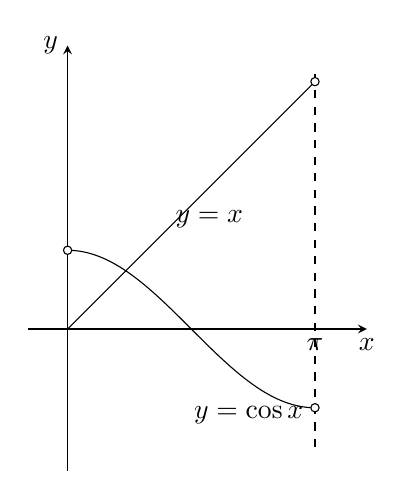
\begin{tikzpicture}[>=stealth,scale=1]
  % axes
  \draw[->] (-0.5,0)--(3.8,0) node[below]{$x$};
  \draw[->] (0,-1.8)--(0,3.6) node[left]{$y$};
  % y = cos x from 0 to pi
  \draw[domain=0:3.1416,samples=100]
      plot (\x,{cos(\x r)});
  \node at (2.3,-1.1) {$y=\cos x$};
  % y = x from 0 to pi
  \draw (0,0)--(3.1416,3.1416);
  \node at (1.8,1.4) {$y=x$};
  % vertical x = pi
  \draw[dashed] (3.1416,-1.5)--(3.1416,3.3);
  \node[below] at (3.1416,0) {$\pi$};
  % open circles
  \filldraw[fill=white] (0,1) circle (1.5pt);      % on cos x at x=0
  \filldraw[fill=white] (3.1416,3.1416) circle (1.5pt);
  \filldraw[fill=white] (3.1416,-1) circle (1.5pt);
\end{tikzpicture}
\end{center}
显然 \(y=x\) 与 \(y=\cos x\) 在 \((0,\pi)\) 上有且仅有唯一交点,即 \(x=\cos x\) 在 \((0,\pi)\) 上有且仅有一个根,而 \(A=\cos A\),\(B=\cos(\cos B)\),由 \(A,B\in(0,\pi)\),所以 \(A=\cos B\),且 \(A=B\),A 对,又\(\frac{\pi}{6}<\cos\frac{\pi}{6}=\frac{\sqrt{3}}{2}\), \(\frac{\pi}{4}>\cos\frac{\pi}{4}=\frac{\sqrt{2}}{2}\), 则\(\frac{\pi}{6}<A=B<\frac{\pi}{4}\),所以\(C=\pi-(A+B)\in(\frac{\pi}{2},\frac{2\pi}{3})\), 即\(B<C\), B 对, C 错,由\(C\in(\frac{\pi}{2},\frac{2\pi}{3})\), 则\(\sin C(\frac{\sqrt{3}}{2},1)\), 而\(C=k\tan(\sin C)\)中\(k>0\),由\(y=\frac{x}{k}\)在区间\((\frac{\pi}{2},\frac{2\pi}{3})\)上单调递增, \(y=\tan(\sin x)\)在区间\((\frac{\pi}{2},\frac{2\pi}{3})\)上单调递减,所以, 只需\(\left\{\frac{\pi}{2k}<\tan 1\right.\), 可得\(\frac{\pi}{2\tan 1}<k<\frac{2\pi}{3}\tan \frac{\sqrt{3}}{2}\),\(\frac{2\pi}{3k}>\tan \frac{\sqrt{3}}{2}\),令\(f(x)=\tan x-x-\frac{x^{3}}{3}\)且\(0<x<\frac{\pi}{2}\), 则\(f'(x)=\frac{1}{\cos^{2}x}-1-x^{2}=1+\tan^{2}x-1-x^{2}=\tan^{2}x-x^{2}\),对于\(g(x)=\tan x-x\)且\(0<x<\frac{\pi}{2}\), 则\(g'(x)=\frac{1-\cos^{2}x}{\cos^{2}x}>0\), 故\(g(x)\)在\((0,\frac{\pi}{2})\)上单调递增,所以\(g(x)>g(0)=0\Rightarrow\tan x>x\), 即\(\tan^{2}x>x^{2}\), 则\(f'(x)>0\),所以\(f(x)\)在\((0,\frac{\pi}{2})\)上单调递增, 故\(f(x)>f(0)=0\), 即\(f(\frac{\sqrt{3}}{2})=\tan \frac{\sqrt{3}}{2}-\frac{\sqrt{3}}{2}-\frac{\sqrt{3}}{8}>0\),所以\(\tan \frac{\sqrt{3}}{2}>\frac{5\sqrt{3}}{8}\), 而\((15\sqrt{3})^{2}=675>64\pi^{2}=(8\pi)^{2}\), 则\(15\sqrt{3}>8\pi\), 即\(\frac{5\sqrt{3}}{8}>\frac{\pi}{3}\),所以\(\tan \frac{\sqrt{3}}{2}>\frac{\pi}{3}\), 故\(\frac{2\pi}{3\tan \frac{\sqrt{3}}{2}}<2\), 即\(k<2\), D 对}
\end{question}

\section{填空题}

\begin{question}
\((1+x)^{5}\)的展开式中\(x^{3}\)项的系数为\_\_\_\_\_\_.
\topics{求指定项的系数}
\difficulty{0.94}
\answer{10}
\explain{\((1+x)^5\)的展开式中\(x^3\)项的系数为\(C_5^3=10\).}
\end{question}

\begin{question}
△ABC 的三个内角A,B,C 的对边分别为a,b,c,满足C=\(\frac{\pi}{4}\),且\(a^{2}+b^{2}-c^{2}=4\),则△ABC 的面积为\_\_\_\_.
\topics{三角形面积公式及其应用;余弦定理解三角形}
\difficulty{0.85}
\answer{1}
\explain{由余弦定理可得:\(c^{2}=a^{2}+b^{2}-2ab\cos\frac{\pi}{4}\),又\(a^{2}+b^{2}-c^{2}=4\),得\(c^{2}=c^{2}+4-\sqrt{2}ab\),解得\(ab=2\sqrt{2}\),所以\(\triangle ABC\)的面积为\(\frac{1}{2}ab\sin C=1\);故答案为:1}
\end{question}

\begin{question}
平面直角坐标系中,原点O处有一只蚂蚁,每过1秒,该蚂蚁都会随机地选择上、下、左、右四个方向之一移动一个单位长度,那么在6秒后,蚂蚁到原点O的距离等于\(\sqrt{2}\)的概率为\_\_\_\_.
\topics{实际问题中的组合计数问题;计算古典概型问题的概率}
\difficulty{0.15}
\answer{\(\frac{75}{256}\)}
\explain{蚂蚁每一秒有4种移动方向,共移动6秒,根据分步乘法计数原理,总路径数为 \(4^{6}\) , 若蚂蚁到原点O的距离为 \(\sqrt{2}\) ,原点(0,0)到该点(x,y)的距离满足 \(x^{2}+y^{2}=2\) , 设蚂蚁右移a次、左移b次,则\(x=a-b\),上移c次、下移d次,则\(y=c-d\),总步数 \(a+b+c+d=6\) , 要满足 \(x^{2}+y^{2}=2\) ,即 \((a-b)^{2}+(c-d)^{2}=2\) ,由于a,b,c,d都是非负整数,可能的组合必须满足 \(|x|=1\) , \(|y|=1\) ,此时, \(a-b=\pm1\) , \(c-d=\pm1\) ,且 \((a+b)+(c+d)=6\) 。设左右移动总次数为\(m=a+b\),上下移动总次数为\(n=c+d\),则\(m+n=6\), 由于\(a=\frac{m+(a-b)}{2}\),\(b=\frac{m-(a-b)}{2}\)需为整数,则\(m\)与\(|a-b|\)同奇偶,所以\(m\)为奇数,同理n也为奇数, 又\(m+n=6\),可能的组合有\(m=1\),\(n=5\)、\(m=3\),\(n=3\)、\(m=5\),\(n=1\), 当\(m=1\),\(n=5\)时,左右移动1次,满足\(|x|=1\)的方式有2种,即左或右, 上下移动5次,满足\(|y|=1\)的方式有\(c=3\),\(d=2\)或\(c=2\),\(d=3\),共\(2\times C_{3}^{3}\)种,即选3次上移,剩下2次下移,或选2次上移,剩下3次下移, 其次,在6步中选1步用于左右移动,其余5步用于上下移动,\(C_{6}^{1}\)种,因此,此情况的路径数为\(C_{6}^{1}\times2\times2\times C_{5}^{3}=240\); 当\(m=3\),\(n=3\)时,左右移动3次,满足\(|x|=1\)的方式有\(a=2\),\(b=1\)或\(a=1\),\(b=2\),共\(2\times C_{3}^{2}\)种,上下移动3次,满足\(|y|=1\)的方式同理,共\(2\times C_{3}^{2}\)种, 此外,6步中选择3步左右移动,剩余上下移动,共\(C_{6}^{3}\)种, 因此,此情况的路径数为\(C_{6}^{3}\times2\times C_{3}^{2}\times2\times C_{3}^{2}=20\times2\times3\times2\times3=720\); 当\(m=5\),\(n=1\)时,与\(m=1\),\(n=5\)对称,路径数为240; 满足条件的总路径数有\(240+720+240=1200\),概率为\(\frac{1200}{4^{6}}=\frac{75}{256}\)。故答案为: \(\frac{75}{256}\) 。}
\end{question}

\section{解答题}

\begin{question}
如图, 六面体 \(ABCD-A_{1}B_{1}C_{1}D_{1}\) 为长方体, \(AB=BC=2\), \(AA_{1}=3\), \(E\), \(F\) 为 \(CC_{1}\) 的三等分点.
\begin{enumerate}
\item 求证:\(D_{1}E\perp AF\);
\item 求直线\(D_{1}E\)与平面\(AA_{1}C_{1}C\)所成角的大小.
\end{enumerate}  

如图, 以 \(A_{1}\) 为坐标原点, 以 \(A_{1}B_{1}\), \(A_{1}D_{1}\), \(A_{1}A\) 分别为 \(x\), \(y\), \(z\) 轴正方向建立空间直角坐标系,

因为 \(AB=BC=2\), \(AA_{1}=3\), \(E\), \(F\) 为 \(CC_{1}\) 的三等分点,

得各点坐标 \(B_{1}\left(2,0,0\right)\), \(D_{1}\left(0,2,0\right)\), \(A\left(0,0,3\right)\), \(E\left(2,2,2\right)\), \(F\left(2,2,1\right)\).

\begin{center}
\begin{tikzpicture}[scale=1]
  % base rectangle (front)
  \coordinate (B1) at (0,0);
  \coordinate (C1) at (3,0);
  \coordinate (D1) at (4,1);
  \coordinate (A1) at (1,1);
  % top rectangle
  \coordinate (B) at ($(B1)+(0,4)$);
  \coordinate (C) at ($(C1)+(0,4)$);
  \coordinate (D) at ($(D1)+(0,4)$);
  \coordinate (A) at ($(A1)+(0,4)$);
  % vertical edges
  \draw (A1)--(A);
  \draw (B1)--(B);
  \draw (C1)--(C);
  \draw (D1)--(D);
  % bottom edges
  \draw (B1)--(C1)--(D1)--(A1)--cycle;
  % top edges
  \draw (B)--(C)--(D)--(A)--cycle;
  % inside dashed edges
  \draw[dashed] (A)--(A1);
  \draw[dashed] (A)--(B1);
  \draw[dashed] (A1)--(C1);
  % segment CE and DF
  \coordinate (E) at ($(C)!0.45!(A1)$);
  \coordinate (F) at ($(D1)!0.45!(A1)$);
  \draw (C)--(E);
  \draw (D1)--(F);
  \draw[dashed] (E)--(A1);
  \draw[dashed] (F)--(A1);
  % labels
  \node[left]  at (B)  {$B$};
  \node[left]  at (B1) {$B_1$};
  \node[above] at (A)  {$A$};
  \node[above] at (D)  {$D$};
  \node[right] at (C)  {$C$};
  \node[right] at (C1) {$C_1$};
  \node[right] at (D1) {$D_1$};
  \node[left]  at (A1) {$A_1$};
  \node[right] at (E)  {$E$};
  \node[right] at (F)  {$F$};
\end{tikzpicture}
\end{center}

\begin{center}
\begin{tikzpicture}[>=stealth,scale=1]
  % base rectangle (front)
  \coordinate (B1) at (0,0);
  \coordinate (C1) at (3,0);
  \coordinate (D1) at (4,1);
  \coordinate (A1) at (1,1);
  % top rectangle (shift up)
  \coordinate (B) at ($(B1)+(0,4)$);
  \coordinate (C) at ($(C1)+(0,4)$);
  \coordinate (D) at ($(D1)+(0,4)$);
  \coordinate (A) at ($(A1)+(0,4)$);
  % axes
  \draw[->] (B1)--(-1,-0.5) node[below]{$x$};
  \draw[->] (D1)--(5,0.5)   node[below]{$y$};
  \draw[->] (A)--(A)+(0,2)  node[above]{$z$};
  % edges
  \draw (B1)--(C1)--(D1)--(A1)--cycle;
  \draw (B)--(C)--(D)--(A)--cycle;
  \draw (A1)--(A);
  \draw (B1)--(B);
  \draw (C1)--(C);
  \draw (D1)--(D);
  % inside dashed edges
  \draw[dashed] (A)--(A1);
  \draw[dashed] (A)--(B1);
  \draw[dashed] (A1)--(C1);
  % segment CE and DF
  \coordinate (E) at ($(C)!0.45!(A1)$);
  \coordinate (F) at ($(D1)!0.45!(A1)$);
  \draw (C)--(E);
  \draw (D1)--(F);
  \draw[dashed] (E)--(A1);
  \draw[dashed] (F)--(A1);
  % labels
  \node[left]  at (B)  {$B$};
  \node[left]  at (B1) {$B_1$};
  \node[above] at (A)  {$A$};
  \node[above] at (D)  {$D$};
  \node[right] at (C)  {$C$};
  \node[right] at (C1) {$C_1$};
  \node[right] at (D1) {$D_1$};
  \node[left]  at (A1) {$A_1$};
  \node[right] at (E)  {$E$};
  \node[right] at (F)  {$F$};
\end{tikzpicture}
\end{center}
\topics{求空间图形上的点的坐标;空间位置关系的向量证明;线面角的向量求法}
\difficulty{0.65}
\answer{(1)证明见解析;(2)\(30^{\circ}\)}
\explain{(1) 以 \(A_{1}\) 为坐标原点建立空间直角坐标系,得 \(\overrightarrow{D_{1}E}=(2,0,2)\),\(\overrightarrow{AF}=(2,2,-2)\),所以 \(\overrightarrow{D_{1}E}\cdot\overrightarrow{AF}=0\),即 \(D_{1}E\perp AF\)。(2) 因为 \(B_{1}D_{1} \perp\) 平面 \(AA_{1}C_{1}C\),所以 \(\overrightarrow{B_{1}D_{1}}=(-2,2,0)\) 为平面法向量,设直线与平面所成角为\(\theta\),则\(\sin\theta=\frac{|\overrightarrow{B_{1}D_{1}}\cdot\overrightarrow{D_{1}E}|}{|\overrightarrow{B_{1}D_{1}}||\overrightarrow{D_{1}E}|}=\frac{4}{2\sqrt{2}\times2\sqrt{2}}=\frac{1}{2}\),所以\(\theta=30^{\circ}\)。}
\end{question}

\begin{question}
某地2021年至2024年新能源汽车销量统计如下表,其中年份代号\(x\)分别为1,2,3,4,销量\(y\)单位为千辆。已知\(\sum_{i=1}^{4} x_{i} y_{i}=966\),\(\sum_{i=1}^{4} \left(y_{i}-\overline{y}\right)^{2}=4896\)。
\begin{enumerate}
\item 试根据样本相关系数\(r\)的值判断该地汽车销量\(y\)与年份代号\(x\)的线性相关性强弱(若\(0.75\leq|r|\leq1\), 则认为\(y\)与\(x\)的线性相关性较强, \(|r|<0.75\), 则认为\(y\)与\(x\)的线性相关性较弱); (精确到0.001)
\item 建立 \(y\) 关于 \(x\) 的线性回归方程,并预测该地 2025 年的新能源汽车销量.
\end{enumerate}
\topics{相关系数的计算;根据回归方程进行数据估计}
\difficulty{0.85}
\answer{(1)\(y\)与\(x\)具有较强的线性相关关系;(2)\(\hat{y}=31.2x+3\),159(千辆)}
\explain{(1) 已知 \(n=4\), \(x_{1}=1, x_{2}=2, x_{3}=3, x_{4}=4\),则 \(\overline{x}=\frac{1+2+3+4}{4}=2.5\), \(y_{1}=33, y_{2}=69, y_{3}=93, y_{4}=129\),则 \(\overline{y}=\frac{33+69+93+129}{4}=81\), \(\sum_{i=1}^{4} x_{i}^{2}=30\), \(4 \overline{x}^{2}=25\),所以 \(\sum_{i=1}^{4} \left(x_{i}-\overline{x}\right)^{2}=5\), 故 \(\sum_{i=1}^{4} \left(x_{i}-\overline{x}\right)\left(y_{i}-\overline{y}\right)=966-4 \times 2.5 \times 81=156\) , 可得 \(r=\frac{156}{\sqrt{5} \times \sqrt{4896}} \approx 0.997\) , 因为 \(|r|=0.997 \geq 0.75\) ,所以 \(y\) 与 \(x\) 具有较强的线性相关关系. (2) \(\hat{b}=\frac{156}{5}=31.2\) , \(\hat{a}=81-31.2 \times 2.5=3\) , 所以 \(\hat{y}=31.2 x+3\) ,将 \(x=5\) 代入得 \(\hat{y}=159\) (千辆).}
\end{question}

\begin{question}
已知数列\(\{a_{n}\}\)和\(\{b_{n}\}\)满足\(a_{1}=1\),\(b_{1}=1\),且\(\left\{\begin{array}{l}a_{n+1}=\frac{1}{2}a_{n}+\frac{3}{2}b_{n} \\ b_{n+1}=\frac{1}{2}b_{n}+\frac{3}{2}a_{n}\end{array}\right.\)。
\begin{enumerate}
\item 证明:数列\(\{a_{n}+b_{n}\}\)与\(\{a_{n}-b_{n}\}\)均为等比数列;
\item 求数列\(\left\{[a_{n}]\right\}\)的前25项和\(S_{25}\).(其中\([x]\)表示不超过\(x\)的最大整数,如\([1.2]=1\))
\end{enumerate}
\topics{由递推关系证明等比数列;求等比数列前n项和;分组(并项)法求和}
\difficulty{0.65}
\answer{(1)证明见解析;(2)\(2^{25}-14\)}
\explain{(1) 由递推关系可得 \(\left\{\begin{array}{l}a_{n+1}+b_{n+1}=2\left(a_{n}+b_{n}\right) \\ a_{n+1}-b_{n+1}=-\left(a_{n}-b_{n}\right)\end{array}\right.\), 又 \(a_{1}+b_{1}=2\neq0, a_{1}-b_{1}=0\neq0\) , 所以 \(\left\{a_{n}+b_{n}\right\}\) 与 \(\left\{a_{n}-b_{n}\right\}\) 均为等比数列。(2) 由(1)知 \(a_{n}+b_{n}=2^{n}\), \(a_{n}-b_{n}=(-1)^{n}\), 所以 \(a_{n}=\frac{2^{n}+(-1)^{n}}{2}\), 则 \([a_{2 n}]=2^{2 n-1}\), \([a_{2 n-1}]=2^{2 n-2}-1\),\(S_{25}=\left(2^{0}-1+2^{1}\right)+\left(2^{2}-1+2^{3}\right)+\cdots+\left(2^{22}-1+2^{23}\right)+2^{24}-1=2^{25}-14\)。}
\end{question}

\begin{question}
已知函数\(f(x)=e^{x}-x-1\)。
\begin{enumerate}
\item 求 \(y=f(x)\) 在 \(x=0\) 处的切线方程;
\item 若 \(f(\ln x)\geq kx-x\ln x-1\) 恒成立, 求实数 \(k\) 的取值范围;
\item 当 \(a\geq1\) 时, 讨论 \(g(x)=f(x)-ax\cos x\) 在区间 \(\left(-\pi,\frac{\pi}{2}\right)\) 上零点的个数.
\end{enumerate}
\topics{求在曲线上一点处的切线方程(斜率);利用导数研究不等式恒成立问题;利用导数研究函数的零点}
\difficulty{0.4}
\answer{(1) \(y=0\);(2)\((-\infty,1]\);(3)3个}
\explain{(1) \(f'(x)=e^{x}-1\),\(f'(0)=f(0)=0\),切线方程为 \(y=0\)。(2) 由\(f(\ln x)\geq kx-x\ln x-1\)得\(x-\ln x-1\geq kx-x\ln x-1\),即\(kx\leq (x-1)\ln x+x\),分离参数得\(k\leq 1+\ln x-\frac{\ln x}{x}\),令\(h(x)=1+\ln x-\frac{\ln x}{x}\),则\(h'(x)=\frac{x+\ln x-1}{x^2}\),\(h(x)\)在\((0,1)\)递减,在\((1,+\infty)\)递增,\(h(x)_{\min}=h(1)=1\),故\(k\in(-\infty,1]\)。(3) 由\(f(0)=0\)知\(x=0\)是零点。当\(x\in(-\frac{\pi}{2},0)\)时,\(g(x)>0\)无零点;当\(x\in(0,\frac{\pi}{2})\)时,\(g'(x)\)先负后正,存在唯一零点;当\(x\in(-\pi,-\frac{\pi}{2})\)时,\(g'(x)>0\),\(g(x)\)单调递增,\(g(-\pi)<0\),\(g(-\frac{\pi}{2})>0\),存在唯一零点。综上,共3个零点。}
\end{question}

\begin{question}
已知平面上两定点\(F_{1}(-2,0)\),\(F_{2}(2,0)\),动点\(P\)满足\(|PF_{1}|\cdot|PF_{2}|=8\),记点\(P\)的轨迹为曲线\(\Gamma\)。设\(M\),\(N\)是曲线\(\Gamma\)与\(x\)轴的两个交点。
\begin{enumerate}
\item 求曲线\(\Gamma\)的方程;
\item 求\(\triangle PMN\)的周长的取值范围;
\item 过\(P\)作直线分别交\(y=\pm x\)于两点\(A,B\),且\(\overrightarrow{AP}=\lambda\overrightarrow{PB}(\lambda>1)\),若\(\triangle OAB\)的面积为18,求\(\lambda\)的最小值.
\end{enumerate}

\begin{center}
\begin{tikzpicture}[>=stealth,scale=1]
  % ellipse
  \draw (0,0) ellipse (3 and 1.5);
  % axes
  \draw[->] (-3.5,0)--(3.8,0) node[below]{$x$};
  \draw[->] (0,-1.8)--(0,2.1) node[left]{$y$};
  % main points
  \coordinate (F1) at (-1.5,0);
  \coordinate (F2) at ( 1.5,0);
  \coordinate (N)  at (-3,0);
  \coordinate (M)  at ( 3,0);
  \coordinate (O)  at ( 0,0);
  \coordinate (P)  at (0,1.5);
  \fill (F1) circle (1pt);
  \fill (F2) circle (1pt);
  \fill (P)  circle (1pt);
  % labels on x-axis
  \node[below] at (N) {$N$};
  \node[below] at (M) {$M$};
  \node[below] at (O) {$O$};
  \node[below] at (F1) {$F_1$};
  \node[below] at (F2) {$F_2$};
  % label P
  \node[above] at (P) {$P$};
\end{tikzpicture}
\end{center}
\topics{利用导数求函数的单调区间(不含参);由方程研究曲线的性质;判断两曲线交点的个数;求平面轨迹方程}
\difficulty{0.15}
\answer{(1)\(\left(x^{2}+y^{2}\right)^{2}-8\left(x^{2}-y^{2}\right)=48\);(2)\(\left[8\sqrt{3}, 4\sqrt{3}+2\sqrt{6+6\sqrt{3}}\right]\);(3)\(2+\sqrt{3}\)}
\explain{(1) 设\(P(x,y)\),则\(\sqrt{(x+2)^2+y^2}\cdot\sqrt{(x-2)^2+y^2}=8\),化简得\(\left(x^2+y^2\right)^2-8\left(x^2-y^2\right)=48\)。(2) 由(1)知\(M\left(2\sqrt{3},0\right)\),\(N\left(-2\sqrt{3},0\right)\),令\(t=x^2+y^2\in[4,12]\),则\(|PM|+|PN|\)关于\(t\)的函数为\(f(t)=t+\sqrt{288-2t^{2}}\),利用导数研究单调性得\(f(t)\)在\([4,4\sqrt{3}]\)递增,在\([4\sqrt{3},12]\)递减,故\(|PM|+|PN|\in[4\sqrt{3},2\sqrt{6+6\sqrt{3}}]\),周长范围为\([8\sqrt{3},4\sqrt{3}+2\sqrt{6+6\sqrt{3}}]\)。
\begin{center}
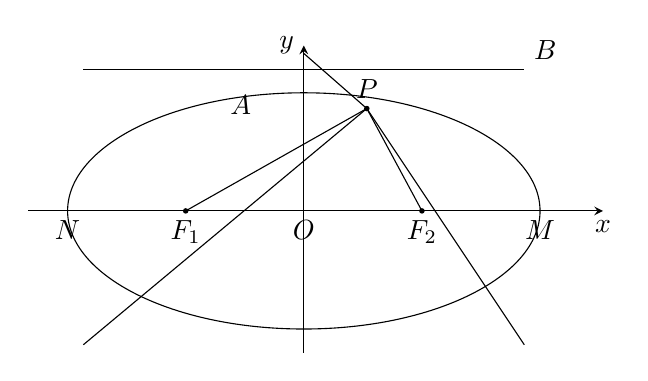
\begin{tikzpicture}[>=stealth,scale=1]
  % ellipse
  \draw (0,0) ellipse (3 and 1.5);
  % axes
  \draw[->] (-3.5,0)--(3.8,0) node[below]{$x$};
  \draw[->] (0,-1.8)--(0,2.1) node[left]{$y$};
  % points on x-axis (foci and ends)
  \coordinate (F1) at (-1.5,0);
  \coordinate (F2) at ( 1.5,0);
  \coordinate (N)  at (-3,0);
  \coordinate (M)  at ( 3,0);
  \coordinate (O)  at ( 0,0);
  \coordinate (P)  at (0.8,1.3);
  \coordinate (A)  at (-0.8,1.1);
  \coordinate (B)  at (2.8,1.8);
  % x-axis labels
  \node[below] at (N) {$N$};
  \node[below] at (M) {$M$};
  \node[below] at (O) {$O$};
  \node[below] at (F1) {$F_1$};
  \node[below] at (F2) {$F_2$};
  % y labels
  \node[above] at (P) {$P$};
  \node[above right] at (B) {$B$};
  \node[above] at (A) {$A$};
  % foci and point P
  \fill (F1) circle (1pt);
  \fill (F2) circle (1pt);
  \fill (P)  circle (1pt);
  % vertical through P
  \draw (P) -- (0,2.0);
  % lines through P
  \draw (F1) -- (P);
  \draw (F2) -- (P);
  \draw (-2.8,1.8) -- (B);
  % another diagonal family
  \draw (-2.8,-1.7) -- (P);
  \draw (2.8,-1.7) -- (P);
\end{tikzpicture}
\end{center}
(3) 设\(A(x_{1},x_{1})\),\(B(x_{2},-x_{2})\),由\(\triangle OAB\)面积为18得\(x_{1}x_{2}=\pm 18\),由\(\overrightarrow{AP}=\lambda\overrightarrow{PB}\)得\(P\left(\frac{x_{1}+\lambda x_{2}}{1+\lambda},\frac{x_{1}-\lambda x_{2}}{1+\lambda}\right)\),代入曲线方程,令\(m=\frac{\lambda}{(1+\lambda)^{2}}\),利用基本不等式求得\(m\leq\frac{1}{6}\),解得\(\lambda\geq 2+\sqrt{3}\),故\(\lambda_{\min}=2+\sqrt{3}\)。}
\end{question}
